% !TeX program = pdflatex
% Сокращённый отчёт для чтения вслух. Собирать из каталога results.
\documentclass[12pt,a4paper]{article}

\usepackage[T2A]{fontenc}
\usepackage[utf8]{inputenc}
\usepackage[russian]{babel}
\usepackage{mathptmx}
\usepackage{tempora}
\usepackage[margin=2cm]{geometry}
\usepackage{setspace}
\usepackage{graphicx}
\usepackage{float}
\usepackage{booktabs}
\usepackage{caption}
\usepackage{indentfirst}
\usepackage{lastpage}

\setstretch{1.25}
\setlength{\parindent}{1.25cm}
\setlength{\parskip}{0pt}
\setlength{\emergencystretch}{3em}
\brokenpenalty=10000
\captionsetup{font=small,labelfont=bf,skip=3pt}
\setlength{\textfloatsep}{10pt plus 2pt minus 2pt}
\setlength{\floatsep}{10pt plus 2pt minus 2pt}
\setlength{\intextsep}{10pt plus 2pt minus 2pt}
\pagestyle{plain}

\begin{document}

\begin{center}
{\Large\bfseries Ширина зерна: программа и штангенциркуль\\
измеряют разные величины\par}
\vspace{0.6em}
{\normalsize 14 ноября 2026 г.\par}
\end{center}

\section{Зачем проверяли и вопрос исследования}

Автоматическая морфометрия зерна обещает быстрый отбор по размеру и форме
[4--6]. Однако перед практическим использованием важно понять, что именно
измеряет программа и можно ли сравнивать её числа со штангенциркулем.
Обычно проверку сводят к корреляции, которая показывает, насколько два
ряда значений связаны, но не показывает, совпадают ли они [1]. Два метода
могут одинаково ранжировать зёрна и при этом давать разные абсолютные
значения, потому что корреляция не чувствительна к постоянному сдвигу и к
разному масштабу. Поэтому в работе проверены и связь, и согласие: смещение,
средняя абсолютная ошибка (MAE), коэффициент согласия Линя (CCC) и пределы
Блэнда--Альтмана [1, 2]. Вопрос исследования простой: какую ширину
вычисляет программа и можно ли её результат считать заменой ручному
замеру? Ответ оказался конкретным: программа считает среднюю хорду, а
штангенциркуль, по принятому допущению, --- максимальную ширину. Эти
величины связаны, но не равны, и их отношение близко к $\pi/4$, поэтому
заметная корреляция может соседствовать с почти нулевым согласием. Такой
результат меняет не оценку качества программы, а постановку задачи: сначала
нужно определить измеряемую величину. Для ширины это особенно заметно: одна
величина описывает максимальный поперечник, другая --- усреднённую хорду.
Работа ограничена шириной; длина, ориентация и калибровка упоминаются
только там, где помогают исключить альтернативные объяснения.

\section{Материал и метод}

Материал --- одна навеска ячменя из 325 зёрен, уложенных в 13 рядов по
25 штук так, что они не касаются друг друга. Сделано восемь снимков одной и
той же навески; по сопроводительным сведениям, состав между кадрами не
менялся, хотя ориентация зёрен менялась. Для каждого зерна есть ручной
замер штангенциркулем, но в файле ручных замеров 324 заполненные строки:
у зерна 275 (ряд 11, позиция 25) замера нет. Прямое сопоставление номера строки и номера
зерна подтверждено структурой рядов, поэтому для согласия используется
324 пары, а для сегментации --- все 325 зёрен.

Ручной эталон, как он используется в работе, --- максимальная ширина, но
протокол замера в файле не описан. Известно только, что значения записаны с
шагом 0,05 мм, и это принято как источник неопределённости, а не как
доказанная методика.

Программа обрабатывает кадр целиком, и параметры не менялись. Сегментация
выделяет светлые зёрна на тёмном фоне, а ширина вычисляется как площадь
выпуклой оболочки, делённая на длину. Вторая ветвь --- короткая сторона
минимального прямоугольника [7] --- ни~разу не сработала, поэтому
экспортируемая ширина является средней хордой. Масштаб в миллиметрах
программа оценивает по линейке в нижней части кадра, и все размеры
пересчитаны по этому масштабу. Для эллипса такая величина равна $\pi/4$ от
максимальной ширины, то есть примерно 0,79. Именно это соотношение
проверяется по данным; на рисунке 1 показан пример разметки.

\begin{figure}[htbp]
\centering
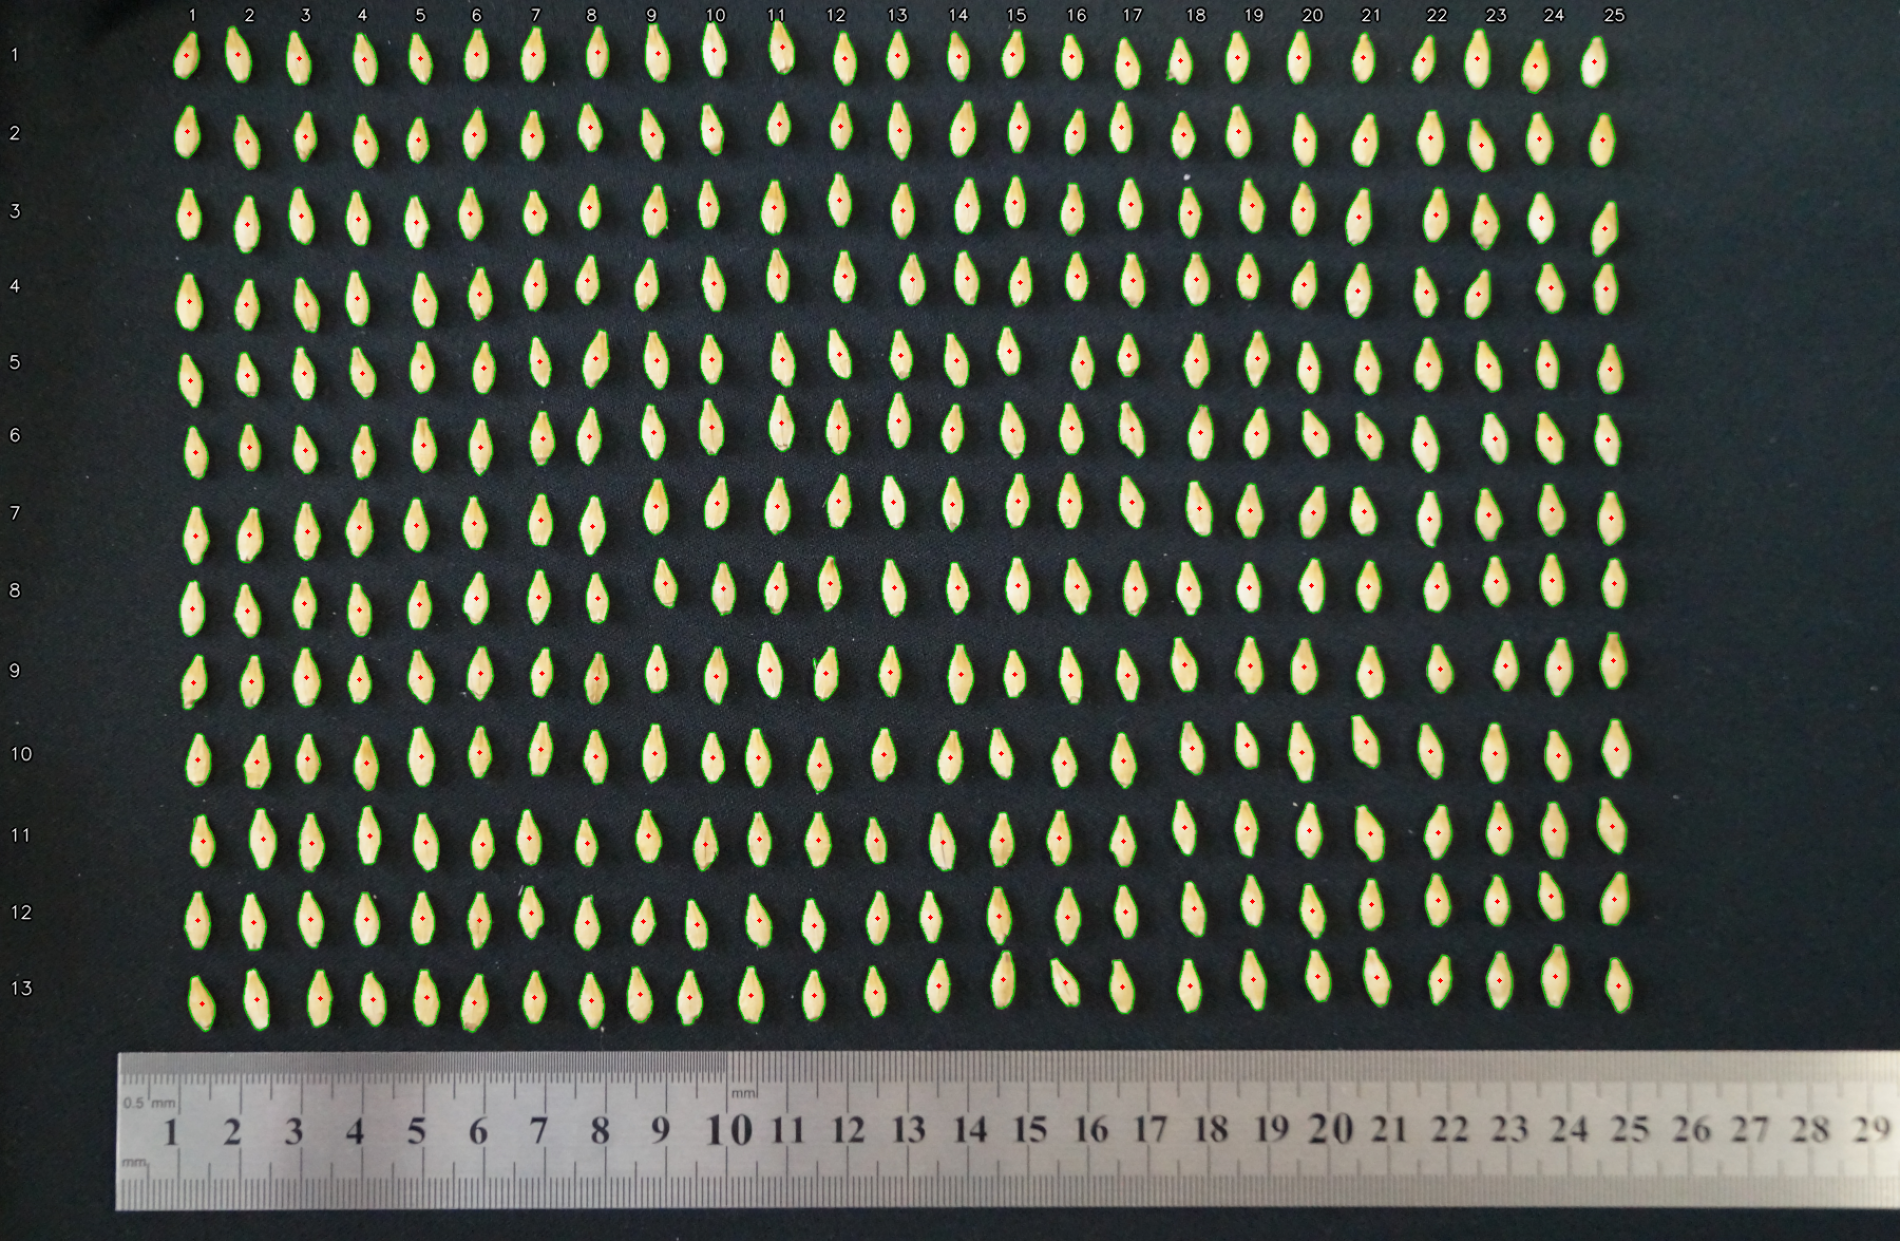
\includegraphics[width=0.75\textwidth]{figures/fig_detection.png}
\caption{Сегментация всех 325 зёрен на одном из восьми снимков; контуры и центры наложены автоматически.}
\label{fig:segmentation}
\end{figure}

Единица анализа --- зерно, а не снимок: восемь кадров являются повторными
измерениями одних и тех же зёрен, поэтому для каждого зерна программа
усреднена по восьми снимкам. Такой расчёт не раздувает выборку, поскольку
восемь кадров не считаются независимыми наблюдениями. Согласие описано
смещением, средней абсолютной ошибкой, корреляцией, коэффициентом согласия
и пределами Блэнда--Альтмана, а повторяемость оценивалась отдельно через
внутриклассовую корреляцию [3]. Для ширины дополнительно проверены
альтернативные геометрические определения.

\section{Результат по ширине}

Средняя ручная ширина --- 3,665 мм, а программа даёт 2,879 мм. Смещение
составляет $-$0,785 мм, и средняя абсолютная ошибка (MAE) равна 0,785 мм.
Это не случайный разброс: пределы согласия лежат от $-$1,105 до $-$0,466
мм, то есть почти все расхождения отрицательны. Корреляция заметная ---
$r = 0{,}636$, но коэффициент согласия Линя (CCC) почти нулевой --- 0,063.
Значит, линейная связь есть, а совпадения значений нет: если бы программа
измеряла максимальную ширину, точки лежали бы вокруг линии равенства.

На рисунке 2 видно, что точки ширины лежат ниже линии равенства, а на
диаграмме Блэнда--Альтмана облако смещено вниз и не пересекает нуль. Это
картина систематического различия, а не случайных выбросов, и отдельные
зёрна показывают тот же эффект. У зерна 302 ручная ширина 4,45 мм, а
программа даёт 2,98 мм; у зерна 266 --- 4,15 и 2,84 мм соответственно. На
этих примерах разрыв особенно заметен.

\begin{figure}[htbp]
\centering
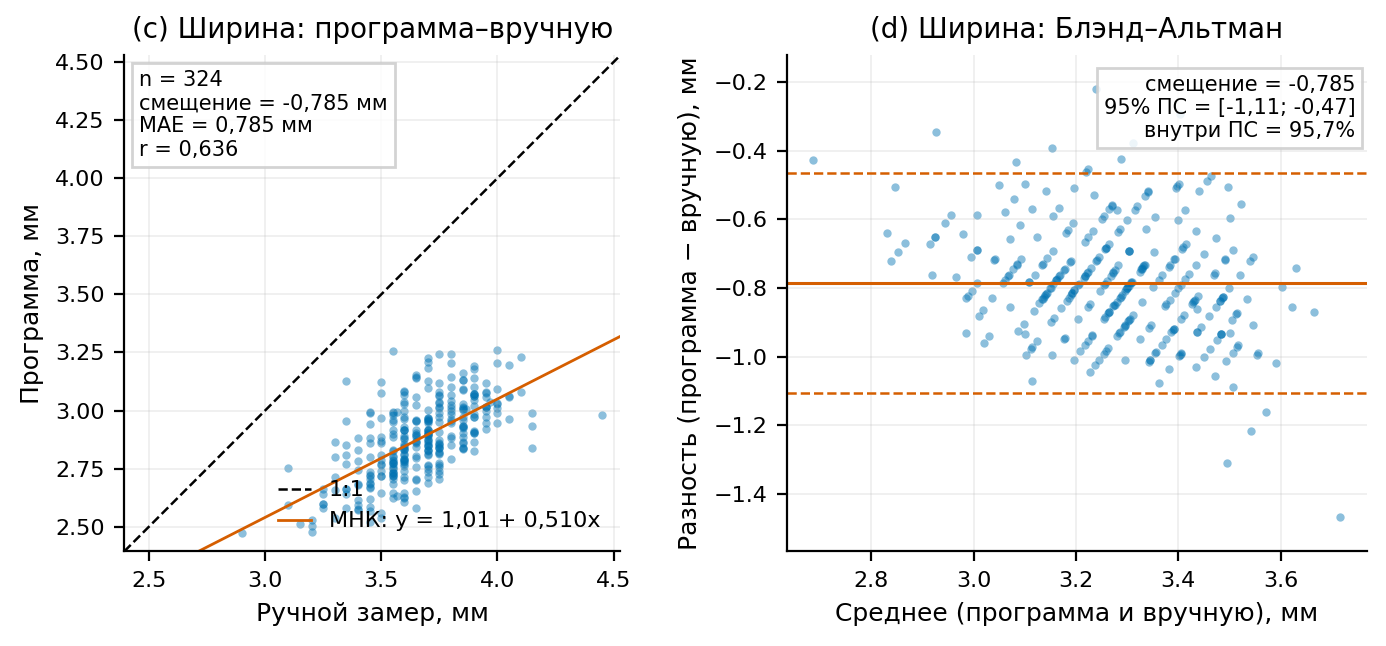
\includegraphics[width=\textwidth]{figures/fig_width_agreement_cd.png}
\caption{Ширина: слева --- рассеяние «программа--вручную», справа --- разности по Блэнду--Альтману; линии показывают смещение и пределы согласия.}
\label{fig:width-agreement}
\end{figure}

Главный количественный аргумент --- отношение: среднее отношение программы
к ручному замеру равно 0,7865, его СКО --- 0,038. Это близко к
$\pi/4 = 0{,}7854$, и формальная проверка не отвергает равенство: $p = 0{,}598$.
Предсказание по ручному среднему составляет 2,878 мм, а фактическое среднее
программы --- 2,879 мм. Совпадение до тысячных не оставляет места для версии
«программа просто ошибается в ширине»: она последовательно измеряет другую
величину. Это не подгонка, потому что коэффициент $\pi/4$ следует из
геометрии эллипса. Средняя хорда и максимальная ширина совпадают только для
прямоугольника; у эллипса они различаются.

Для эллипса площадь пропорциональна произведению полуосей, а длина ---
большой оси. Если разделить площадь на длину, получается $\pi/4$ от
максимальной ширины, и именно это наблюдается. Реальное зерно не эллипс:
бороздка, неровный край и несимметричный контур немного меняют отношение.
Поэтому разброс 0,038 --- не дефект, а следствие формы, хотя среднее значение
держится у $\pi/4$. На рисунке 3 схема и реальное зерно показывают это
соотношение.

\begin{figure}[tbp]
\centering
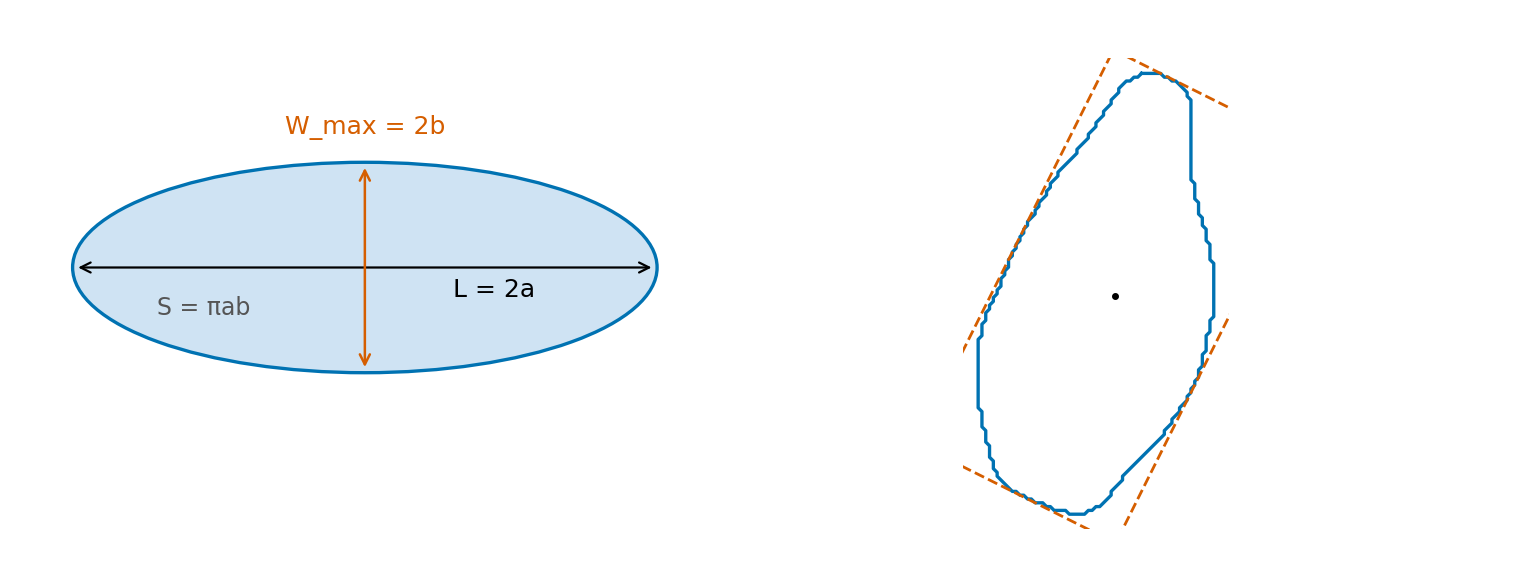
\includegraphics[width=0.95\textwidth]{figures/fig_width_definition_clean.png}
\caption{Слева --- эллипс, справа --- реальное зерно: длина и максимальная ширина; для эллипса отношение средней хорды к максимальной ширине равно $\pi/4$.}
\label{fig:width-definition}
\end{figure}

Проверка альтернативных определений подтверждает диагноз: если взять
короткую сторону минимального прямоугольника, смещение становится
+0,321 мм. MAE при этом 0,325 мм, а корреляция 0,681, тогда как поперечная
протяжённость даёт +0,364 мм. Обе величины гораздо ближе к ручной
максимальной ширине, чем экспортируемая средняя хорда. Это не результат
программы, а диагностика: те же контуры, другое определение, и смена
определения почти убирает смещение. Оба определения ближе к максимальной
ширине, но не совпадают с ней. Эти определения не заменяют экспортируемую
величину, а объясняют её.

\pagebreak[4]
Таблица 1 сводит два определения: экспортируемая средняя хорда даёт
смещение $-$0,785 мм, а короткая сторона минимального прямоугольника ---
+0,321 мм. Разница между ними и есть цена определения. Для пользователя это
практический вывод. Если нужна максимальная ширина, текущую формулу нельзя
сравнивать со штангенциркулем напрямую; если нужна средняя ширина, она
осмысленна, но требует своего эталона. Сначала нужно выбрать величину,
потом сравнивать методы, иначе валидация будет измерять разницу определений,
а не качество программы. Максимальная ширина удобна для сравнения со
штангенциркулем, средняя хорда --- для площади и формы.

\begin{table}[htbp]
\centering
\small
\caption{Два определения ширины: смещение относительно ручного эталона}
\label{tab:width-def}
\begin{tabular}{@{}lrrr@{}}
\toprule
Определение & Смещение, мм & MAE, мм & $r$ \\
\midrule
Средняя хорда (экспорт) & $-$0,785 & 0,785 & 0,636 \\
Короткая сторона minAreaRect & +0,321 & 0,325 & 0,681 \\
\bottomrule
\end{tabular}
\end{table}

\section{Почему это не ошибка сегментации и не калибровка}

Первое подозрение --- сегментация, но на всех восьми снимках программа
нашла 325 зёрен из 325, и повторный прогон дал те же числа. Проверка
структуры важна: программа могла бы найти 325 объектов, но перепутать ряды.
Однако контуры устойчивы, и структура 13 рядов по 25 позиций
восстанавливается без сдвигов. Если бы контур захватывал соседнее зерно или
терял край, ширина менялась бы хаотично, а вместо этого отношение держится
у $\pi/4$. Значит, программа видит те же объекты, но измеряет у них другую
величину.

Второе подозрение --- калибровка, но проверка по штрихам линейки дала
расхождение до 2,1 \%, а среднее --- $-$0,3 \%. Такой масштаб не объясняет
смещение 0,785 мм, потому что ошибка калибровки меняет все размеры
пропорционально, а здесь отношение стабильно. Именно стабильность отношения
исключает масштабную ошибку, поэтому калибровка не является причиной.

Третье подозрение --- общая ошибка обработки. Для длины смещение +0,342
мм, корреляция длины --- 0,953, а CCC длины --- 0,781. Длина тоже не
идеальна, но она ведёт себя как размер: связь сильная, смещение умеренное.
Ширина выпадает из этой картины, и если бы программа плохо сегментировала,
пострадали бы обе величины. Разрыв между длиной и шириной указывает на
определение, а не на отказ обработки, хотя контуры общие.

Наконец, альтернативные определения: короткая сторона прямоугольника даёт
+0,321 мм, а поперечная протяжённость --- +0,364 мм. Это почти ручная
максимальная ширина, и те же контуры с другой формулой меняют смещение на
миллиметр. Значит, вопрос не в качестве сегментации и не в калибровке, а в
том, что именно считается шириной. Вывод не «программа плохая», а
«программа отвечает на другой вопрос»; это не оправдание, а уточнение
задачи.

\section{Ограничения}

Ограничения начинаются с материала: проверена одна навеска, одна серия и
восемь снимков, а зёрна, по сообщению оператора, целые и не касаются друг
друга. Переносить вывод на другие сорта, навески, разрешения, освещение или на слипшиеся зёрна нельзя.
Даже для этой навески отношение 0,7865 является средним, потому что у
отдельных зёрен оно варьирует из-за формы. Вывод относится к целым зёрнам
этой навески, а не к сорту в целом.

Второе ограничение --- ручной эталон: протокол замера отсутствует, и
неизвестно, сколько раз мерили, один ли оператор работал и как выбиралась
максимальная ширина. Шаг записи --- 0,05 мм, хотя заявленное округление не
совпадает с фактическим шагом. Часть различия может относиться к эталону, а
не к программе, ведь ручной эталон мог измеряться с другой повторяемостью.
Поэтому вывод сформулирован как различие величин, а не как ошибка одной
стороны.

Третье ограничение --- влажность и условия съёмки: влажность не
измерялась, а происхождение образца и условия хранения не предоставлены.
Восемь снимков --- повторные измерения, а не независимые наблюдения; для
согласия использовано 324 зерна, для сегментации --- 325. Наконец, $\pi/4$ ---
приближение для эллипса, и для реального зерна с бороздкой отношение немного
ниже, поэтому точное значение 0,7865 нельзя считать универсальной
константой. Для других условий нужна отдельная проверка, так что результат
--- не метрологическая аттестация, а сравнение в данных условиях.

\section{Вывод и что делать дальше}

Программа и штангенциркуль измеряют разные величины ширины: программа
возвращает среднюю хорду, а ручной эталон, по принятому допущению, ---
максимальную ширину. Их отношение близко к $\pi/4$, поэтому корреляция
может быть заметной, а согласие --- почти нулевым, и сравнивать значения
напрямую нельзя. Главный вывод: корреляция не заменяет проверку согласия, а
для практики нужен протокол, в котором ширина определена до измерения.

Чтобы получить максимальную ширину, нужно изменить формулу или ввести
пересчёт, проверенный на независимой выборке. Если нужна средняя ширина,
текущая величина осмысленна, но её эталон должен быть другим, ведь
максимальная ширина --- это отдельный признак. Следующий шаг ---
зафиксировать в протоколе, какая именно ширина нужна, и добавить в программу
оба определения. Тогда сравнение со штангенциркулем станет корректным, а
выбор метрики --- осознанным и воспроизводимым для других исследователей;
иначе разница определений снова будет выглядеть как ошибка. Проверку стоит повторить на независимой навеске с
документированным ручным протоколом: она покажет, устойчиво ли отношение
$\pi/4$. До этого вывод остаётся ограниченным данной серией. Такой протокол
снизит риск повторной путаницы между определением величины и качеством
измерения.

\renewcommand{\refname}{Список литературы}
{\small
\setstretch{1.0}
\begin{thebibliography}{7}
\setlength{\itemsep}{0pt}

\bibitem{bland1986}
Bland J.M., Altman D.G. Statistical methods for assessing agreement between
two methods of clinical measurement // The Lancet. 1986. Vol.~327, no.~8476.
P.~307--310.

\bibitem{lin1989}
Lin L.I.-K. A concordance correlation coefficient to evaluate
reproducibility // Biometrics. 1989. Vol.~45, no.~1. P.~255--268.

\bibitem{shrout1979}
Shrout P.E., Fleiss J.L. Intraclass correlations: uses in assessing rater
reliability // Psychological Bulletin. 1979. Vol.~86, no.~2. P.~420--428.

\bibitem{tanabata2012}
Tanabata T., Shibaya T., Hori K., Ebana K., Yano M. SmartGrain:
high-throughput phenotyping software for measuring seed shape through image
analysis // Plant Physiology. 2012. Vol.~160, no.~4. P.~1871--1880.

\bibitem{li2014}
Li L., Zhang Q., Huang D. A review of imaging techniques for plant
phenotyping // Sensors. 2014. Vol.~14, no.~11. P.~20078--20111.

\bibitem{symons1988}
Symons S.J., Fulcher R.G. Determination of wheat kernel morphological
variation by digital image analysis: I. Variation in Eastern Canadian
milling quality wheats // Journal of Cereal Science. 1988. Vol.~8, no.~3.
P.~211--218.

\bibitem{igathinathane2008}
Igathinathane C., Pordesimo L.O., Columbus E.P., Batchelor W.D.,
Methuku S.R. Shape identification and particles size distribution from
basic shape parameters using ImageJ // Computers and Electronics in
Agriculture. 2008. Vol.~63, no.~2. P.~168--182.

\end{thebibliography}
}

\end{document}
